%
%%%%%%%%%%%%%%%%%%%%%%%%%%%%%%%%%%%%%%%%%%%%%%%%%%%
%
%  E N T W I C K L U N G S U M G E B U N G
%
%%%%%%%%%%%%%%%%%%%%%%%%%%%%%%%%%%%%%%%%%%%%%%%%%%%
\chapter{Entwicklungsumgebung}
\label{cha:umgebung}
%
%
Wer gerne lokal mit eigener LaTeX-Installation arbeitet, verwendet beipsielsweise als Entwicklungsumgebung unter Windows die Kombination aus MiKTeX\footnote{www.miktex.org} und TeXstudio\footnote{texstudio.sourceforge.net/}. Auf heise.de\footnote{www.heise.de/software} kann man auch drekt das TeXstudio als Portable-Version herunterladen, die nicht einmal installiert werden muss und auf jedem USB-Stick Platz findet.\\

Laden und installieren Sie zunächst MiKTeX, dann installieren oder öffnen Sie das TeXstudio. Laden Sie die Haupt-.tex-Datei der Abschlussarbeit. Auf der linken Seite sollten nun auch alle Einzelkapitel, Anhänge und das Glossar angezeigt werden. Durch drücken des grünen Doppelpfleils in der Icon-Leiste wird das fertige .pdf erstellt und direkt im Studio angezeigt. Außerdem liegt das fertige .pdf natürlich auch im Projektordner.\\

Zum Bearbeiten eines Kapitels Ihrer Abschlussarbeit drücken Sie einfach im linken Struktur-Fenster auf das entsprechende Kapitel und editieren Sie den Inhalt.\\ 

Wer lieber online arbeitet, sei Overleaf (de.overleaf.com) empfohlen. Hier legt man sich per Registrierung einen eigenen Zugang an und kann dort dann im Netz arbeiten.\\
Auch hier sollte die oben genannte Struktur verwendet werden: Hauptdokument im Projektverzeichnis, pro Kapitel ein entsprechender Ordner mit der zugehörigen .tex-Datei und eventuell dort jeweils ein Bildordner (siehe Menü auf der linken Seite in Abbildung \ref{fig:overleaf}). 
%
\begin{figure}
  \centering
   {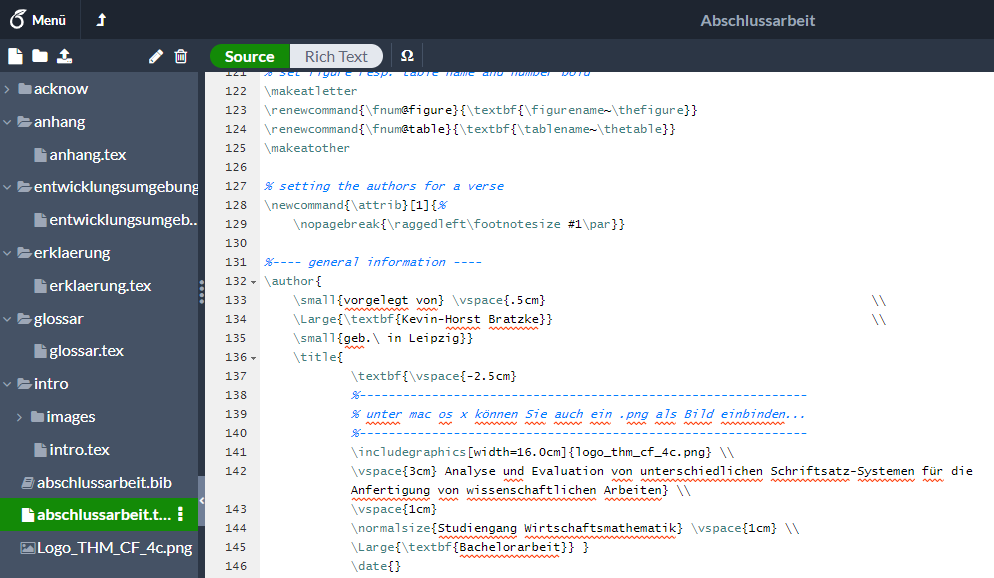
\epsfig{file = entwicklungsumgebung/images/overleaf_screenshot.png, width=14.6cm}}
  \caption[Overleaf]{Screenshot des Overleaf Webinterface mit Quelltext und Dokumenten-Anzeige.}
  \label{fig:overleaf}
\end{figure}
%
